\section{Dominio físico}
El dominio físico es la transformación de las funciones que el sistema debe desempeñar en componentes físicos. Estos pueden ser partes, ensambles, módulos, dispositivos, sistemas.

La representación del dominio físico es mediante un diagrama a bloques, denominado arquitectura funcional, con base en las funciones generadas de un sistema mecatrónico, se propone la siguiente arquitectura. 

\begin{figure}[h!]
    \centering
        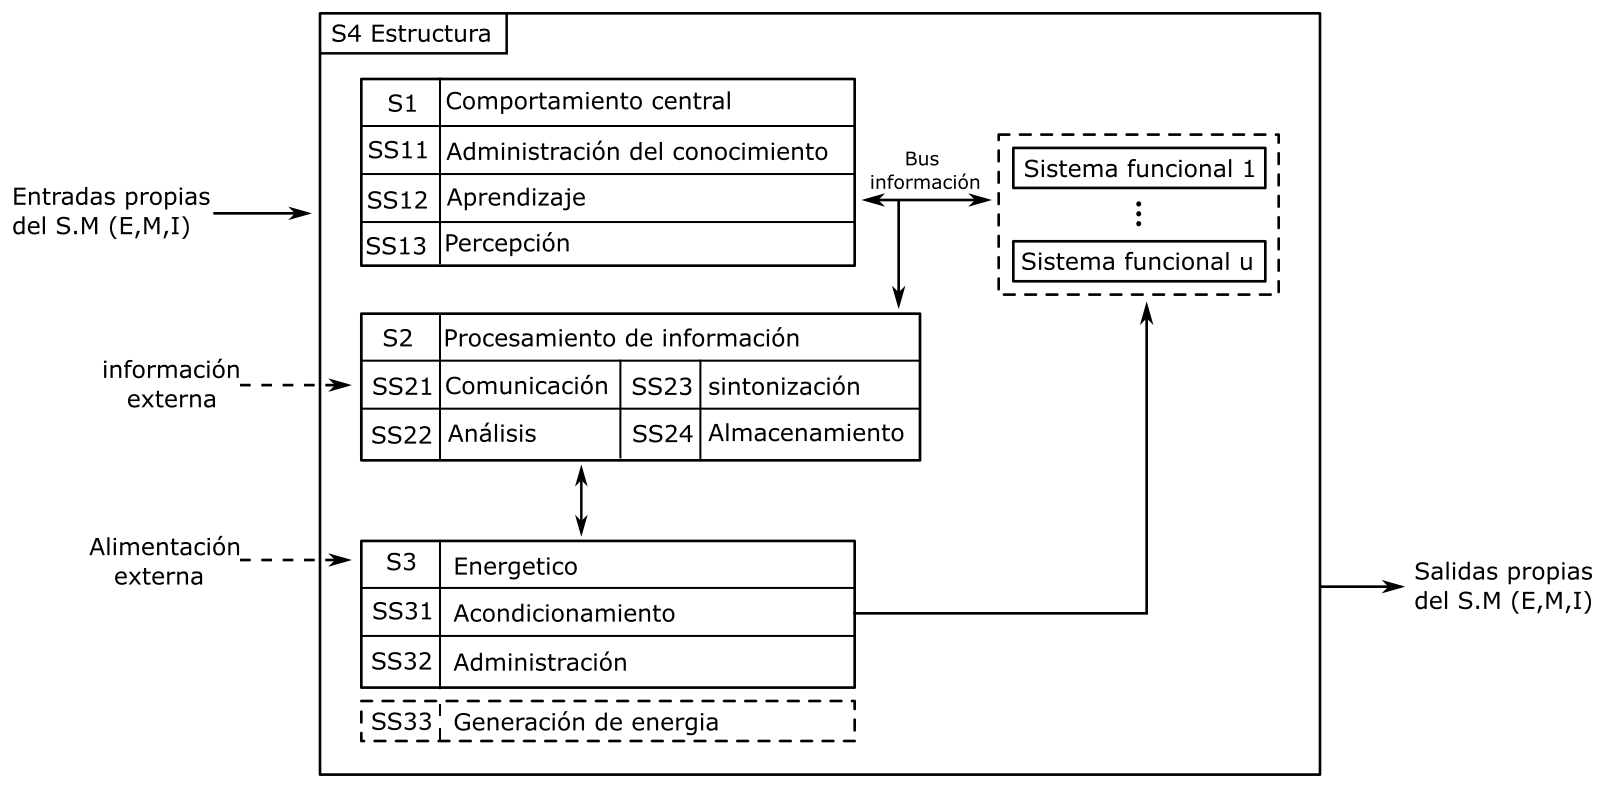
\includegraphics[scale=0.22]{Proyecto Integrador Figuras/22 Dominio fisico.png}
        \caption{Dominio físico}
\end{figure}

Con base en teoría de sistemas, un sistema mecatrónico se puede considerar como un "sistema de sistemas" (SoS), y a su vez el sistema que tiene mayor impacto en el sistema mecatrónico se denomina como "sistema de interés" (SoI).

\begin{figure}[h!]
    \centering
        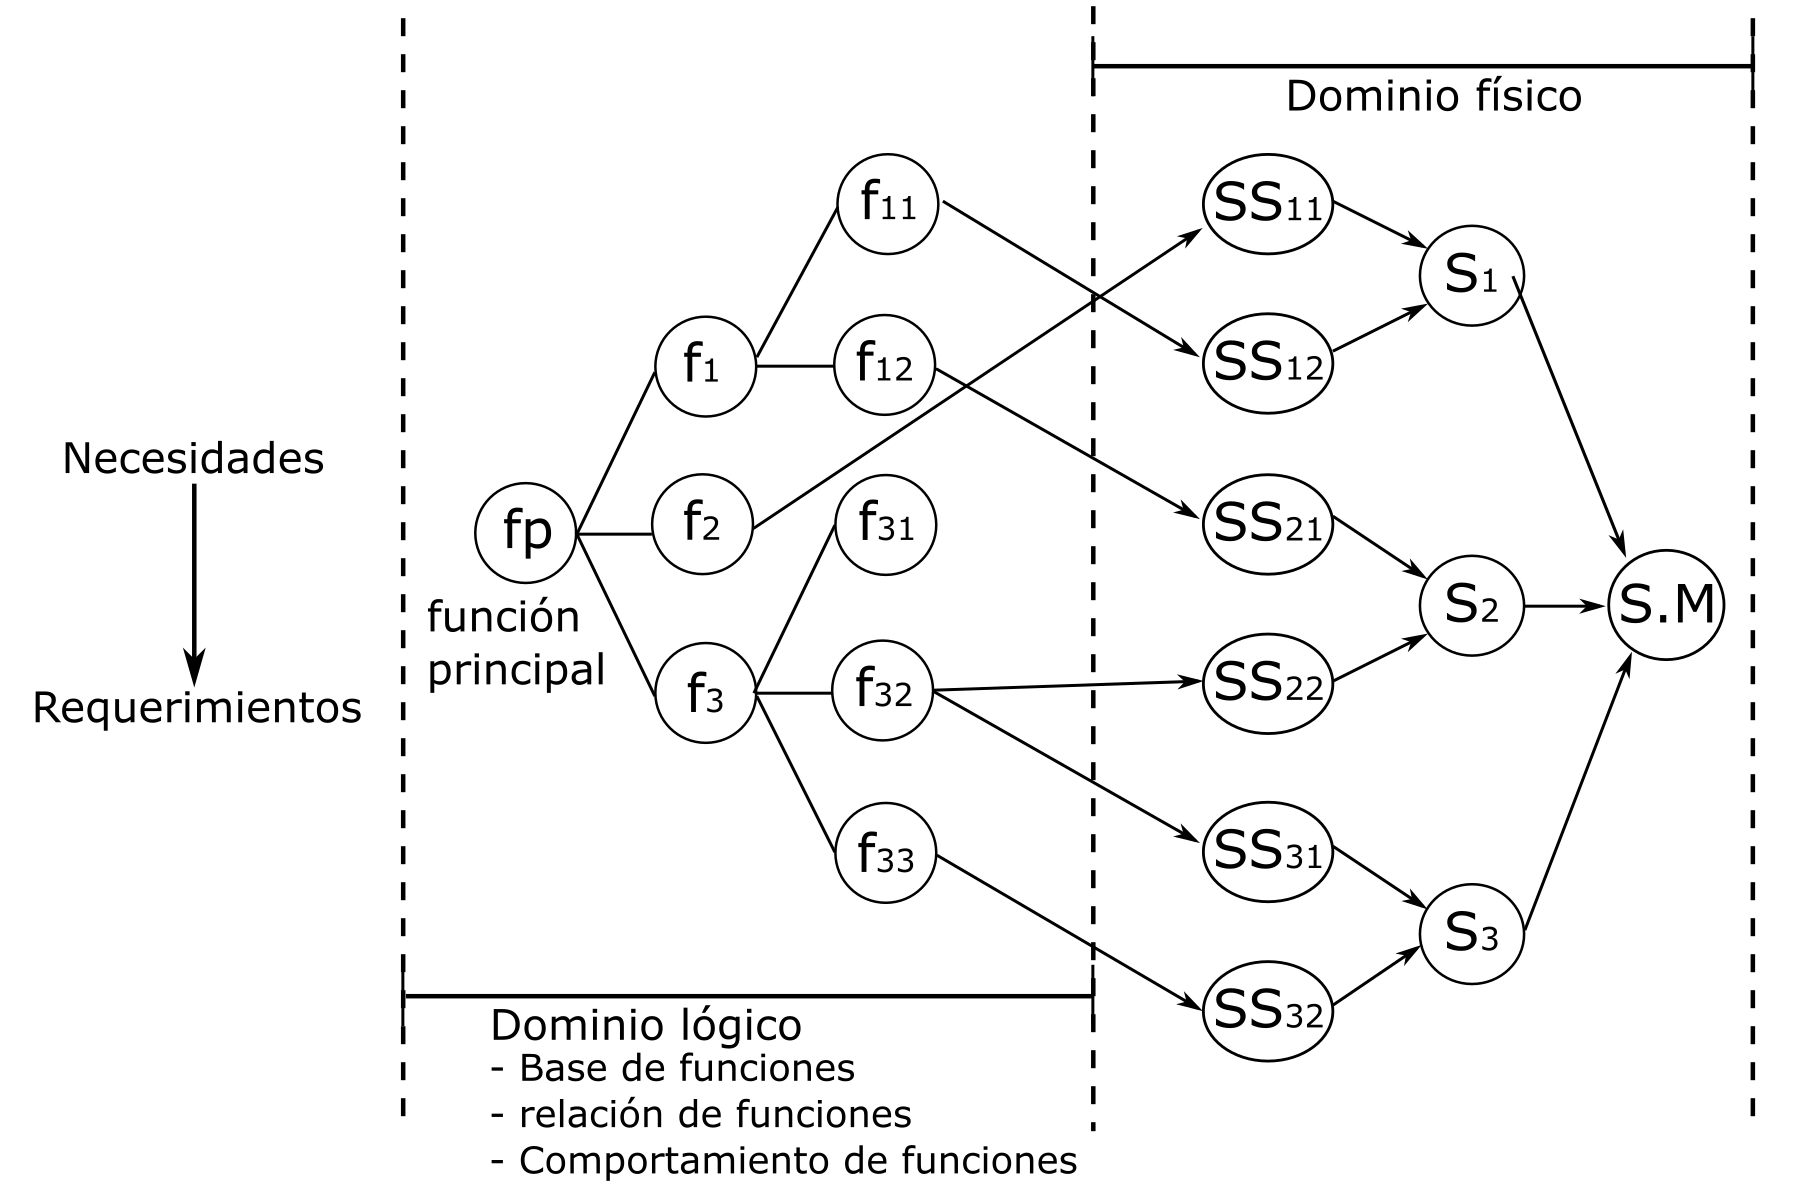
\includegraphics[scale=0.20]{Proyecto Integrador Figuras/23 Dominio Logico y Fisico.png}
        \caption{Dominio lógico y físico}
\end{figure}